% Telos shared preamble.
%
% Every Telos publication is designed to be printed on a home laser printer,
% one sheet at a time, and carried into a boat or a garage. Two constraints
% follow from that and govern everything below:
%
%   1. Pure monochrome. No value is ever a hue. Emphasis is carried by rule
%      weight, fill, and type, never by color, so a grayscale or black-only
%      printer loses nothing.
%   2. Card density. A "one-pager" is a hard contract: the leaf must fit on a
%      single side of US Letter. The layout is therefore tight by default and
%      the environments below are sized to leave room for a plate.

\documentclass[10pt,letterpaper]{article}

\usepackage[margin=0.55in,includefoot,footskip=0.24in]{geometry}
\usepackage[T1]{fontenc}
\usepackage[utf8]{inputenc}
\usepackage{lmodern}
\usepackage{microtype}
\usepackage{array}
\usepackage{booktabs}
\usepackage{longtable}
\usepackage{tabularx}
\usepackage{enumitem}
\usepackage{needspace}
\usepackage{multicol}
\usepackage{ragged2e}
\usepackage{graphicx}
\usepackage{wrapfig}
\usepackage{xcolor}
\usepackage{fancyhdr}
\usepackage{titlesec}
\usepackage{hyperref}
\usepackage[most]{tcolorbox}
\usepackage{tikz}
\usetikzlibrary{arrows.meta,calc,positioning,shapes.geometric,decorations.pathmorphing,patterns,fadings}

% Semantic names are kept so a document reads intelligibly, but every value is
% black, white, or a neutral gray that survives a black-only print driver.
\definecolor{telosink}{gray}{0}
\definecolor{telospaper}{gray}{1}
\definecolor{telosrule}{gray}{0.35}
\definecolor{telosfill}{gray}{0.90}
\definecolor{telosdeep}{gray}{0.72}
\definecolor{telosmute}{gray}{0.45}

\hypersetup{hidelinks,pdfborder={0 0 0}}

% Keep an unchanged source byte-reproducible across rebuilds: no build-clock
% creation date and no random trailer ID.
\pdfinfoomitdate=1
\pdftrailerid{}

\setlength{\parindent}{0pt}
\setlength{\parskip}{0.42em}
\setlength{\tabcolsep}{4pt}
\setlength{\columnsep}{1.1em}
\renewcommand{\arraystretch}{1.18}
\setlist[itemize]{leftmargin=1.15em,itemsep=0.12em,topsep=0.2em,parsep=0pt}
\setlist[enumerate]{leftmargin=1.5em,itemsep=0.18em,topsep=0.2em,parsep=0pt}
\setlist[description]{leftmargin=0pt,itemsep=0.16em,topsep=0.2em,parsep=0pt,
  font=\normalfont\bfseries}

% ---------------------------------------------------------------------------
% Document identity. Each leaf declares these before \begin{document} so the
% running head, the colophon, and the PDF metadata all agree.
% ---------------------------------------------------------------------------
\newcommand{\TelosProject}{Telos}
\newcommand{\TelosDocTitle}{}
\newcommand{\TelosDocSubtitle}{}
\newcommand{\TelosRevision}{}

\newcommand{\telosmeta}[4]{%
  \renewcommand{\TelosProject}{#1}%
  \renewcommand{\TelosDocTitle}{#2}%
  \renewcommand{\TelosDocSubtitle}{#3}%
  \renewcommand{\TelosRevision}{#4}%
  \hypersetup{pdftitle={#2},pdfsubject={#3; version #4},
    pdfkeywords={Telos, version #4},pdfauthor={Telos}}%
}

\pagestyle{fancy}
\fancyhf{}
\renewcommand{\headrulewidth}{0pt}
\renewcommand{\footrulewidth}{0.4pt}
\fancyfoot[L]{\footnotesize\textsc{\TelosProject}}
\fancyfoot[C]{\footnotesize\TelosDocTitle}
\fancyfoot[R]{\footnotesize\thepage}

% The first page of a one-pager carries the masthead instead of a running foot,
% so its footer is the compact provenance line.
\fancypagestyle{telosfirst}{%
  \fancyhf{}%
  \renewcommand{\headrulewidth}{0pt}%
  \renewcommand{\footrulewidth}{0.4pt}%
  \fancyfoot[L]{\footnotesize\textsc{\TelosProject}}%
  \fancyfoot[C]{\footnotesize\TelosRevision}%
  \fancyfoot[R]{\footnotesize\thepage}%
}

% ---------------------------------------------------------------------------
% Masthead. A heavy rule, the title, a light subtitle, a thin rule. The
% optional argument is a right-aligned tag (a species' scientific name, a
% lesson number) that sits on the title's baseline.
% ---------------------------------------------------------------------------
\newcommand{\telosmasthead}[1][]{%
  \thispagestyle{telosfirst}%
  \begingroup
  \setlength{\parskip}{0pt}%
  \noindent\rule{\linewidth}{1.6pt}\par
  \vspace{0.30em}
  \noindent
  \begin{minipage}[b]{0.66\linewidth}
    \raggedright{\LARGE\bfseries\TelosDocTitle}
  \end{minipage}%
  \hfill
  \begin{minipage}[b]{0.32\linewidth}
    \raggedleft{\small\itshape #1}
  \end{minipage}\par
  \vspace{0.18em}
  \noindent{\small\TelosDocSubtitle}\par
  \vspace{0.28em}
  \noindent\rule{\linewidth}{0.4pt}\par
  \endgroup
  \vspace{0.35em}
}

% ---------------------------------------------------------------------------
% Headings. Compact, small-caps, rule-anchored — a card has no room for the
% article class's default vertical air.
% ---------------------------------------------------------------------------
\titleformat{\section}{\normalfont\large\bfseries}{}{0pt}{}[\vspace{-0.55em}\rule{\linewidth}{0.4pt}]
\titlespacing*{\section}{0pt}{0.85em}{0.35em}
\titleformat{\subsection}{\normalfont\normalsize\bfseries}{}{0pt}{}
\titlespacing*{\subsection}{0pt}{0.6em}{0.2em}
\titleformat{\subsubsection}{\normalfont\small\bfseries\scshape}{}{0pt}{}
\titlespacing*{\subsubsection}{0pt}{0.45em}{0.12em}

% A short run-in heading for card interiors that must not consume a full line.
\newcommand{\telosrubric}[1]{\textbf{#1}\enspace}

% Cross-reference helper. Every Telos project is a set of loose printed sheets,
% so a reference names the sheet rather than a page number.
\newcommand{\sheetref}[1]{\textit{see the \textbf{#1} sheet}}

% Which decision, ADR or sheet governs the paragraph you are reading. A reader
% who disagrees with an instruction should be able to find the reasoning behind
% it rather than having to take it on trust.
\newcommand{\governedby}[1]{{\footnotesize\textsc{governed by #1}}}

% ---------------------------------------------------------------------------
% Quantities. siunitx is not in this TeX Live split, and the guides need only a
% fixed thin space and upright units, so define that directly rather than take
% a package dependency the documented install would not satisfy.
%   \qty{9}{kV}  ->  9 kV        \unitof{kV}  ->  kV
% ---------------------------------------------------------------------------
\newcommand{\unitof}[1]{\ensuremath{\mathrm{#1}}}
\newcommand{\qty}[2]{#1\,\unitof{#2}}
\newcommand{\numrange}[2]{#1\,--\,#2}
\newcommand{\qtyrange}[3]{#1\,--\,#2\,\unitof{#3}}
% Inches and feet appear constantly in the fishing guide; keep one spelling.
\newcommand{\inch}[1]{#1\,in}
\newcommand{\feet}[1]{#1\,ft}

% ---------------------------------------------------------------------------
% Cards and boxes.
% ---------------------------------------------------------------------------

% Titled card with a hairline frame. The default card for facts a reader looks
% up rather than reads through.
\newtcolorbox{teloscard}[1]{
  enhanced, breakable,
  colback=telospaper, colframe=telosink, colbacktitle=telospaper,
  coltitle=telosink,
  boxrule=0.5pt, sharp corners,
  left=6pt, right=6pt, top=4pt, bottom=4pt,
  toptitle=3pt, bottomtitle=3pt, titlerule=0.4pt,
  before skip=6pt, after skip=6pt,
  title={#1}, fonttitle=\small\bfseries
}

% Untitled left-ruled block: hierarchy without a redundant label.
\newtcolorbox{telosframe}{
  enhanced, breakable,
  colback=telospaper, frame hidden, boxrule=0pt, sharp corners,
  borderline west={1.3pt}{0pt}{telosink},
  left=8pt, right=2pt, top=3pt, bottom=3pt,
  before skip=6pt, after skip=6pt
}

% Filled emphasis panel — the "read this first" block. The 10% fill stays
% legible under a cheap laser toner curve and still reads as distinct.
\newtcolorbox{telospanel}[1]{
  enhanced, breakable,
  colback=telosfill, colframe=telosink, colbacktitle=telosfill,
  coltitle=telosink,
  boxrule=0.5pt, sharp corners,
  left=6pt, right=6pt, top=4pt, bottom=4pt,
  toptitle=3pt, bottomtitle=3pt, titlerule=0.4pt,
  before skip=6pt, after skip=6pt,
  title={#1}, fonttitle=\small\bfseries
}

% Hazard block. Deliberately the heaviest object on any page: a 1.4pt frame
% plus a solid title bar. Nothing else in Telos is allowed to look like this,
% so a reader skimming a lesson cannot mistake it for ordinary emphasis.
\newtcolorbox{teloshazard}[1]{
  enhanced, breakable,
  colback=telospaper, colframe=telosink,
  colbacktitle=telosink, coltitle=telospaper,
  boxrule=1.4pt, sharp corners,
  left=6pt, right=6pt, top=5pt, bottom=5pt,
  toptitle=3pt, bottomtitle=3pt,
  before skip=8pt, after skip=8pt,
  title={\MakeUppercase{#1}}, fonttitle=\small\bfseries
}

% A stop-and-check gate. Used before anything destructive, and before anything
% that would be expensive to discover later. Shared by every project that has
% a procedure someone could get hurt following carelessly.
\newtcolorbox{gate}[1]{
  enhanced, breakable,
  colback=telospaper, colframe=telosink,
  boxrule=1.0pt, sharp corners,
  left=6pt, right=6pt, top=4pt, bottom=4pt,
  toptitle=3pt, bottomtitle=3pt, titlerule=0.4pt,
  before skip=7pt, after skip=7pt,
  colbacktitle=telospaper, coltitle=telosink,
  title={\MakeUppercase{#1}}, fonttitle=\small\bfseries
}

% ---------------------------------------------------------------------------
% Rating dots. A five-step scale that prints identically in black-only: filled
% versus open circles, never a shaded bar.
% ---------------------------------------------------------------------------
\newcommand{\telosdot}{\tikz[baseline=-0.42ex]\fill[telosink] (0,0) circle (0.28ex);}
\newcommand{\telosopendot}{\tikz[baseline=-0.42ex]\draw[telosink,line width=0.28pt] (0,0) circle (0.28ex);}
\makeatletter
\newcounter{telos@rate}
\newcommand{\telosrating}[1]{%
  \begingroup
  \setcounter{telos@rate}{0}%
  \@whilenum\value{telos@rate}<#1\do{\telosdot\kern0.22em\stepcounter{telos@rate}}%
  \@whilenum\value{telos@rate}<5\do{\telosopendot\kern0.22em\stepcounter{telos@rate}}%
  \endgroup
}
\makeatother

% ---------------------------------------------------------------------------
% Tables.
%
% tabularx reads its body by scanning for a literal \end{tabularx}, so it can
% never be wrapped in a \newenvironment. Documents therefore open tabularx and
% longtable directly and take their house style from these column types and the
% booktabs rules. The one exception is the fact strip below, which is built on
% plain tabular precisely so it *can* be an environment.
% ---------------------------------------------------------------------------
\newcolumntype{L}{>{\raggedright\arraybackslash}X}
\newcolumntype{R}{>{\raggedleft\arraybackslash}X}
\newcolumntype{C}{>{\centering\arraybackslash}X}
\newcolumntype{B}{>{\bfseries\raggedright\arraybackslash}X}
\newcolumntype{N}{>{\raggedright\arraybackslash}p{0.16\linewidth}}

% Key/value fact strip. Two flush columns of short lookups; the label column is
% a fixed fraction so a stack of cards aligns across the whole guide.
\newenvironment{telosfacts}[1][0.24]
  {\begingroup\small
   \setlength{\parskip}{0pt}%
   \renewcommand{\arraystretch}{1.25}%
   \begin{tabular}{@{}>{\bfseries\raggedright\arraybackslash}p{\dimexpr#1\linewidth\relax}@{\hspace{0.7em}}>{\raggedright\arraybackslash}p{\dimexpr\linewidth-#1\linewidth-0.7em\relax}@{}}}
  {\end{tabular}\par\endgroup}
\newcommand{\telosfact}[2]{#1 & #2\\}

% ---------------------------------------------------------------------------
% Seasonal / diurnal activity bar.
%
% \telosseasonbar{4,3,2,1,1,2,3,3,4,5,4,3} draws a twelve-cell month strip
% where each value 0-5 is a fill height. Height, not gray value, carries the
% signal, so it is exact under any toner curve; the cell is outlined either way
% so an empty month is still visibly a month.
% ---------------------------------------------------------------------------
\newcommand{\telosseasonlabels}{J,F,M,A,M,J,J,A,S,O,N,D}
\newcommand{\telosseasonbar}[1]{%
  \begingroup
  \begin{tikzpicture}[x=1.25em,y=2.1ex,baseline=0pt]
    \foreach \v [count=\i from 0] in {#1} {
      \draw[telosrule,line width=0.3pt] (\i,0) rectangle (\i+0.86,5);
      \ifnum\v>0
        \fill[telosink] (\i,0) rectangle (\i+0.86,\v);
      \fi
    }
    \foreach \m [count=\i from 0] in \telosseasonlabels {
      \node[font=\tiny,anchor=north,inner sep=1.2pt] at (\i+0.43,-0.1) {\m};
    }
  \end{tikzpicture}%
  \endgroup
}

% Four-cell day-part strip: dawn, midday, dusk, night.
\newcommand{\telosdaylabels}{Dawn,Mid,Dusk,Night}
\newcommand{\telosdaybar}[1]{%
  \begingroup
  \begin{tikzpicture}[x=2.9em,y=2.1ex,baseline=0pt]
    \foreach \v [count=\i from 0] in {#1} {
      \draw[telosrule,line width=0.3pt] (\i,0) rectangle (\i+0.92,5);
      \ifnum\v>0
        \fill[telosink] (\i,0) rectangle (\i+0.92,\v);
      \fi
    }
    \foreach \m [count=\i from 0] in \telosdaylabels {
      \node[font=\tiny,anchor=north,inner sep=1.2pt] at (\i+0.46,-0.1) {\m};
    }
  \end{tikzpicture}%
  \endgroup
}

% A bar needs vertical room for its labels when it sits in a fact strip.
\newcommand{\telosbarrow}[1]{\rule{0pt}{4.2ex}#1\rule[-1.6ex]{0pt}{1.6ex}}

% ---------------------------------------------------------------------------
% Plates. A species or apparatus illustration with a caption rule beneath it.
% \telosplate{width fraction}{file}{caption}
% ---------------------------------------------------------------------------
\newcommand{\telosplate}[3]{%
  \begingroup
  \centering
  \includegraphics[width=#1\linewidth]{#2}\par
  \vspace{0.15em}
  \begin{minipage}{#1\linewidth}
    \rule{\linewidth}{0.4pt}\par
    \vspace{0.1em}
    {\footnotesize #3\par}
  \end{minipage}\par
  \endgroup
  \vspace{0.3em}
}

% TikZ drawing conventions shared by every rig, knot, and circuit diagram.
\tikzset{
  telos line/.style={draw=telosink,line width=0.7pt},
  telos hair/.style={draw=telosink,line width=0.35pt},
  telos heavy/.style={draw=telosink,line width=1.2pt},
  telos node/.style={draw=telosink,fill=telospaper,align=center,inner sep=4pt,font=\small},
  telos emphasis/.style={draw=telosink,line width=1.2pt,fill=telospaper,align=center,
    inner sep=4pt,font=\small\bfseries},
  telos label/.style={font=\scriptsize,inner sep=1.5pt},
  telos arrow/.style={-{Stealth[length=1.8mm]},draw=telosink,line width=0.6pt},
  telos dim/.style={|<->|,draw=telosink,line width=0.35pt},
  telos water/.style={draw=telosrule,line width=0.4pt,decorate,
    decoration={snake,amplitude=0.4mm,segment length=3mm}},
}

% ---------------------------------------------------------------------------
% Lesson furniture
% ---------------------------------------------------------------------------

% \lessonhead{number}{time}{who does what}
\newcommand{\lessonhead}[3]{%
  \par\noindent
  \begin{minipage}{\linewidth}
    \rule{\linewidth}{0.4pt}\par
    \vspace{0.3em}
    {\small\textbf{Lesson #1}\quad$\cdot$\quad #2\quad$\cdot$\quad #3\par}
    \vspace{0.25em}
    \rule{\linewidth}{0.4pt}
  \end{minipage}\par
  \vspace{0.5em}}

% The materials list. Two columns of short lines; a lesson that needs a long
% shopping list is a lesson that has not been thought through.
\newenvironment{materials}
  {\begin{telospanel}{What you need}\begin{multicols}{2}
   \begin{itemize}[leftmargin=1em,itemsep=0.05em,topsep=0pt]}
  {\end{itemize}\end{multicols}\end{telospanel}}

% The four rubrics every lesson carries, in the same order every time:
% what you are about to see, what to do, what it means, and what to ask.
\newcommand{\lessonsection}[1]{\section*{#1}\vspace{-0.35em}\rule{\linewidth}{0.4pt}\vspace{0.2em}}

% A prediction box. The point of the curriculum is that they commit to an
% answer before the demonstration, not after.
\newtcolorbox{predict}{
  enhanced, breakable,
  colback=telospaper, colframe=telosink,
  boxrule=0.5pt, sharp corners,
  left=6pt, right=6pt, top=4pt, bottom=4pt,
  before skip=6pt, after skip=6pt,
  borderline west={2.2pt}{0pt}{telosink},
  title={\small\bfseries Predict first}, fonttitle=\small\bfseries,
  colbacktitle=telospaper, coltitle=telosink,
  toptitle=3pt, bottomtitle=3pt, titlerule=0.4pt,
}

% ---------------------------------------------------------------------------
% Colophon. Rendered once, at the end of the last page, in the recovered footer
% area so it never creates a page of its own.
% ---------------------------------------------------------------------------
\newif\ifTelosColophonRendered
\newcommand{\TelosColophonExtra}{}
\newcommand{\TelosColophon}{%
  \ifTelosColophonRendered\else
  \global\TelosColophonRenderedtrue
  \par
  \enlargethispage{0.5in}%
  \vspace{0.3em}%
  \begingroup
  \setlength{\parskip}{0pt}%
  \begin{minipage}{\linewidth}
  \rule{\linewidth}{0.35pt}\par
  \vspace{0.3em}%
  \fontsize{7}{8.2}\selectfont
  \textbf{Telos.} \TelosProject{} — \TelosDocTitle. Revised \TelosRevision.
  \TelosColophonExtra{}
  Project-created text and diagrams are licensed \href{https://creativecommons.org/licenses/by/4.0/}{CC BY 4.0}.
  Incorporated public-domain artwork remains public domain and is credited on
  the plate it appears with. See \texttt{LICENSE} and \texttt{CREDITS.md} in the
  source. Nothing here is professional advice; verify current regulations and
  follow the stated safety procedure.
  \end{minipage}
  \endgroup
  \fi
}
\AtEndDocument{\TelosColophon}

% Shared macros for the homelab project.
%
% This project's documents are read in two very different situations: at a desk
% while designing, and standing in front of a broken machine at eleven at night
% with no network. The second case is the one that sets the style. Commands are
% set apart so they can be found by eye, every dangerous step has a visible
% verification after it, and nothing depends on being able to reach a web page.

% ---------------------------------------------------------------------------
% Decision-record entries, used by the generated digest.
% ---------------------------------------------------------------------------
\newcommand{\adrentry}[4]{%
  \par\vspace{0.7em}
  \needspace{4\baselineskip}%
  \noindent
  \begin{minipage}{\linewidth}
    \rule{\linewidth}{0.6pt}\par
    \vspace{0.25em}
    {\small\textbf{ADR #1}\quad #2\par}
    \vspace{0.1em}
    {\fontsize{7}{8.2}\selectfont\textsc{#3}\quad$\cdot$\quad #4\par}
    \vspace{0.2em}
    \rule{\linewidth}{0.3pt}
  \end{minipage}\par
  \vspace{0.3em}}

% ---------------------------------------------------------------------------
% Procedures.
%
% A rebuild manual is a sequence of commands and the observable evidence that
% each one worked. These environments keep that pairing structural rather than
% a matter of the author remembering.
% ---------------------------------------------------------------------------

% A block of shell to type. Deliberately not a listing package: plain verbatim
% in a ruled box prints identically everywhere and has no font dependency.
\newenvironment{shellblock}
  {\par\vspace{0.25em}\noindent
   \begin{minipage}{\linewidth}
   \rule{\linewidth}{0.3pt}\par\vspace{0.15em}
   \begingroup\footnotesize\ttfamily\obeylines\obeyspaces\parindent=0pt\parskip=0pt}
  {\endgroup\par\vspace{0.15em}\rule{\linewidth}{0.3pt}\end{minipage}\par\vspace{0.25em}}

% What you should see if the previous step worked. A step without one of these
% is a step you cannot verify, and in a rebuild manual that is a defect.
\newcommand{\expectthis}[1]{%
  \par\vspace{0.1em}
  \noindent\begin{minipage}{\linewidth}
  \hspace*{0.6em}\begin{minipage}{\dimexpr\linewidth-0.6em\relax}
  {\footnotesize\textbf{Expect:} #1\par}
  \end{minipage}\end{minipage}\par\vspace{0.3em}}

% \begin{gate} now lives in common/preamble.tex, shared with the other
% projects that document procedures.

% \governedby now lives in common/preamble.tex.

% An instance value that comes from the private overlay. In the published
% documents these render as visible placeholders, which is deliberate: a
% published manual must be complete and obviously generic, never look like it
% is describing somebody's actual network.
\newcommand{\instancevalue}[2]{\texttt{\textlangle #1\textrangle}%
  \footnote{Instance value. Supplied from \texttt{homelab/instance/} at build
  time; #2.}}
\newcommand{\placeholder}[1]{\texttt{\textlangle #1\textrangle}}

% ---------------------------------------------------------------------------
% Role and boundary diagrams.
% ---------------------------------------------------------------------------
\tikzset{
  role/.style={draw=telosink,line width=0.9pt,fill=telospaper,align=center,
    inner sep=5pt,font=\small,minimum width=2.6cm},
  roleoff/.style={draw=telosmute,line width=0.5pt,dash pattern=on 2.5pt off 1.8pt,
    fill=telospaper,align=center,inner sep=5pt,font=\small,minimum width=2.6cm},
  boundary/.style={draw=telosmute,line width=0.5pt,dash pattern=on 3pt off 2pt,
    rounded corners=3pt},
  flow/.style={-{Stealth[length=2mm]},draw=telosink,line width=0.7pt},
  hlabel/.style={font=\fontsize{6.4}{7.4}\selectfont},
}


\telosmeta{Homelab}{Controller Design}
  {What the Controller is, what it owns, and what it deliberately does not}{20260725.001}

\begin{document}
\telosmasthead[High-level design]

The Controller is the homelab's infrastructure host. It answers DHCP and DNS for
its managed network, serves the boot chain that installs every other machine,
and is the one system that must be reconstructible without any other system
being available. Everything else in the lab may depend on the Controller. The
Controller may depend on nothing except a copy of this document, an installer
image and a recorded set of inputs.

\section{Scope}
\begin{telosfacts}[0.22]
\telosfact{It owns}{Boot, storage and encryption; the managed network interface; bundled DHCPv4 and \texttt{home.arpa} DNS; PXE selection and first-stage TFTP; the HTTP artifact service; local recovery; and its own checkpoint and rollback.}
\telosfact{It may host}{The optional Services role --- Homebridge, openHAB and similar --- and the identity domain controller in a VM. Both are separable and neither is required for the Controller to do its job. \governedby{ADR 0054, ADR 0055}}
\telosfact{It does not do}{Routing, NAT or perimeter firewalling. It has one network interface and advertises no default route. On the isolated acceptance network there is deliberately no path to the Internet. \governedby{ADR 0011}}
\telosfact{It is not}{A hypervisor-first platform. Foundational services run directly on the Arch host; containers and VMs are used where they earn their place, not by default. \governedby{ADR 0014}}
\telosfact{One failure domain}{Containers and VMs on the Controller share its hardware, its kernel maintenance window and its power supply. Placing a service on the Controller does not make it independently available.}
\end{telosfacts}

\section{Roles and boundaries}
\begin{center}
\begin{tikzpicture}[
  x=1cm,y=1cm,scale=1.12,every node/.append style={transform shape},
  graphite/.style={draw=telosink,line width=0.55pt,
    preaction={draw=telosmute,line width=1.15pt,opacity=.16}},
  graphite heavy/.style={draw=telosink,line width=0.9pt,
    preaction={draw=telosmute,line width=1.65pt,opacity=.18}},
  hatch/.style={draw=telosmute,line width=0.25pt,opacity=.62},
  card/.style={draw=telosink,line width=0.5pt,fill=telospaper,
    rounded corners=.4pt,align=left,inner xsep=5pt,inner ysep=4pt,
    font=\fontsize{6.4}{7.3}\selectfont},
  wire/.style={-{Stealth[length=1.6mm]},draw=telosink,line width=0.55pt},
  note/.style={font=\fontsize{5.8}{6.7}\selectfont,align=left},
]
  % The slight doubled strokes and hand hatching survive ordinary office printing.
  \draw[graphite heavy,rounded corners=2pt] (-.25,-2.88) rectangle (6.15,2.68);
  \draw[hatch] (-.12,2.46) -- (.12,2.60) (.18,2.46) -- (.42,2.60)
    (.48,2.46) -- (.72,2.60) (.78,2.46) -- (1.02,2.60);
  \node[anchor=west,font=\fontsize{7}{8}\selectfont\bfseries] at (.05,2.27)
    {CONTROLLER \textnormal{· Arch host · ADR 0015}};

  % Front-panel hardware cues anchor the service map in one physical failure domain.
  \draw[graphite] (.08,-2.61) rectangle (.34,-2.35);
  \fill[telosink] (.21,-2.48) circle (.035);
  \draw[graphite] (.48,-2.56) rectangle (.83,-2.40);
  \foreach \y in {-2.33,-2.42,-2.51,-2.60}
    \foreach \x in {5.25,5.43,5.61,5.79}
      \draw[hatch] (\x,\y) -- ++(.11,.06);

  \node[card,text width=2.15cm] (net) at (1.43,1.20)
    {\textbf{dnsmasq}\\DHCP · \texttt{home.arpa} DNS\\PXE selection · TFTP};
  \node[card,text width=2.15cm] (http) at (4.72,1.20)
    {\textbf{nginx}\\signed install artifacts\\manifest and checksums};
  \node[card,text width=2.15cm] (boot) at (1.43,-.28)
    {\textbf{systemd-boot}\\three signed UKIs\\one complete rescue image};
  \node[card,text width=2.15cm] (store) at (4.72,-.28)
    {\textbf{LUKS2 + Btrfs}\\system checkpoint\\separate mutable state};
  \node[card,dashed,text width=2.15cm,text=telosmute] (svc) at (1.43,-1.72)
    {\textbf{Services role}\\Podman quadlets\\optional · stopped};
  \node[card,dashed,text width=2.15cm,text=telosmute] (dir) at (4.72,-1.72)
    {\textbf{Samba AD DC}\\separate VM boundary\\optional · stopped};

  \draw[wire] (boot.east) -- (store.west);
  \node[note,anchor=south] at (3.08,-.22) {encrypted root};
  \draw[wire] (net.east) -- (http.west);
  \node[note,anchor=south] at (3.08,1.26) {artifacts};
  \draw[wire,dashed,telosmute] (svc.east) -- (dir.west);

  % One and only one physical network jack leaves the chassis.
  \draw[graphite heavy] (6.15,.58) -- (6.54,.58);
  \draw[graphite] (6.28,.45) rectangle (6.54,.71);
  \node[note,anchor=south] at (6.4,.76) {\texttt{lan0}};
  \draw[wire] (6.54,.58) -- (7.28,.58);
  \draw[graphite] (7.28,.19) -- (7.28,.97) -- (8.12,.58) -- cycle;
  \foreach \y in {.36,.58,.80}
    \draw[graphite] (7.48,\y) -- (7.72,\y);
  \node[note,anchor=south] at (7.68,1.03) {isolated switch};

  \draw[wire] (8.12,.58) -- (8.72,1.45);
  \draw[wire] (8.12,.58) -- (8.72,-.28);
  \draw[graphite heavy] (8.72,1.15) rectangle (10.08,1.92);
  \draw[graphite] (9.24,1.03) -- (9.56,1.03) (9.4,1.03) -- (9.4,.91);
  \node[note,anchor=south] at (9.4,1.31) {Workstation};
  \draw[graphite heavy,rounded corners=1pt] (8.83,-.72) rectangle (9.97,.12);
  \draw[graphite] (9.09,-.57) rectangle (9.71,-.44);
  \node[note,anchor=south] at (9.4,-.30) {Client};

  \node[note,anchor=north west,text width=3.3cm] at (6.63,-1.12)
    {\textbf{Deliberate absence}\\No router, NAT, perimeter firewall, or advertised default route.};
  \draw[graphite] (6.67,-2.08) -- (9.83,-2.08);
  \node[note,anchor=north west,text width=3.3cm,text=telosmute] at (6.63,-2.16)
    {Dashed cards are relocatable roles; both are disabled by default.};
\end{tikzpicture}
\end{center}

\section{Storage}
\begin{tabularx}{\linewidth}{@{}p{0.10\linewidth}p{0.16\linewidth}L@{}}
\toprule
\textbf{Part} & \textbf{Size} & \textbf{Why}\\
\midrule
ESP & 2 GiB, FAT32 & systemd-boot plus three UKIs, one of which carries a complete rescue userspace. Sized with deliberate headroom so an update can stage a full new artifact set before switching. The ESP is the one partition that cannot be grown afterwards without moving everything behind it. \governedby{ADR 0051}\\
Root & remainder, LUKS2 & Btrfs inside the encrypted container. The operating system is one checkpointable subvolume; logs, caches, home directories, the snapshot store and mutable service data are separate subvolumes excluded from it. \governedby{ADR 0026, ADR 0027}\\
Swap & file in root & A file inside the encrypted Btrfs, so encrypted swap costs no second LUKS container. Hibernation is disabled --- a machine whose job is answering DHCP does not suspend.\\
\bottomrule
\end{tabularx}

There is no Windows partition. ADR 0047 removed it: firmware maintenance uses
\texttt{fwupd} where the vendor publishes to LVFS and vendor-supplied bootable
media otherwise, which costs nothing until the day it is needed and removes a
licence, a BitLocker recovery-key custody chain and a second Secure Boot trust
path from the design.

\section{The network boundary}
\begin{telosfacts}[0.22]
\telosfact{One interface}{Selected explicitly at install time and pinned by permanent MAC address to the stable name \texttt{lan0}. There is no default and no automatic choice, because binding DHCP to the wrong link puts a second DHCP authority on a network the Controller does not own. \governedby{ADR 0050}}
\telosfact{One authority}{dnsmasq is the only address-assigning DHCP server on its layer-2 network. Where external infrastructure owns DHCP, the Controller's instance stays stopped. Two authorities on one segment is forbidden at every stage, including transitions. \governedby{ADR 0008, ADR 0044}}
\telosfact{Bundled}{DHCP and DNS start and stop as one unit. A partial success is a failure. \governedby{ADR 0012}}
\telosfact{IPv4 only}{Managed addressing is IPv4. The host's IPv6 stack stays enabled and unmanaged; nothing globally disables it. \governedby{ADR 0013}}
\telosfact{Four inputs}{The operator supplies subnet, Controller address, and pool start and end. Netmask, network and broadcast addresses, the DNS server, the suffix and the absence of a router are all derived. Contradictory values cannot reach dnsmasq because they cannot be entered. \governedby{ADR 0045}}
\telosfact{Fail closed}{First boot verifies the interface, its MAC, carrier, the address and the absence of a competing DHCP authority before starting anything. If any check fails, DHCP stays stopped and the machine reports why. \governedby{ADR 0009}}
\end{telosfacts}

\section{Lifecycle: install once, converge continuously}
The single most important structural decision is that installation and
configuration are different things with different cadences.

\begin{tabularx}{\linewidth}{@{}p{0.17\linewidth}L@{}}
\toprule
\textbf{Stage} & \textbf{What happens}\\
\midrule
Install & Only what cannot be done later: partition, encrypt, make filesystems, install the base system and both kernels, write boot artifacts, configure \texttt{lan0} and the static address, install \texttt{sshd} with the administrator public key, record the manifest. Then power off. \governedby{ADR 0010, ADR 0053}\\
Relocate & The operator physically moves the powered-off Controller to the isolated switch. Being powered off during the move is the primary DHCP-conflict safety boundary --- not a configuration flag. \governedby{ADR 0010}\\
First boot & One-shot activation validates the network plan, then starts dnsmasq and nginx together, or leaves them stopped and says why.\\
Converge & Everything else is Ansible over SSH from this repository: package sets, service configuration, the Services role, identity client, users, sudo, health checks. Idempotent, reviewable as a diff, and the same mechanism for the Controller and every Workstation. \governedby{ADR 0053}\\
Update & Guarded: read the news, checkpoint, full-system upgrade, reboot if foundational, validate DHCP, DNS and PXE automatically, roll back if validation fails. \governedby{ADR 0016, ADR 0028}\\
\bottomrule
\end{tabularx}

\begin{telospanel}{Why this split matters}
The previous design specified provisioning in detail and day-two configuration
not at all, which meant that adding a service or changing a DHCP reservation
implied reinstalling the machine. Nothing iterates at that cost, so in practice
the running system drifts from the record and the record stops being true. The
install stage is deliberately small so that it can be fully tested; everything
that changes often lives where changes are cheap and reversible.
\end{telospanel}

\section{State model: prove each boundary before crossing it}
\begin{center}
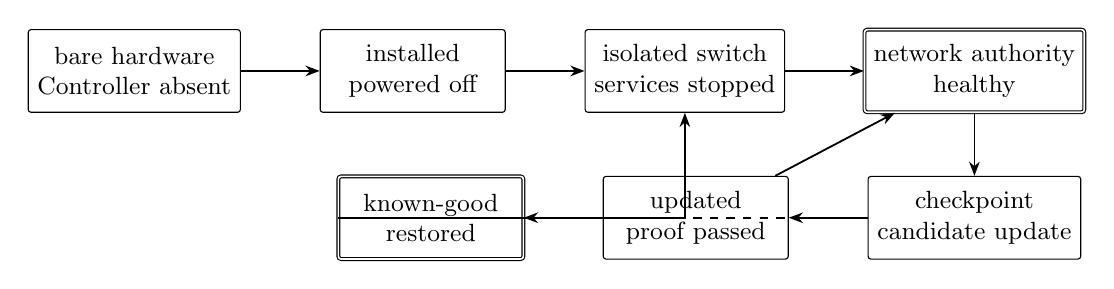
\begin{tikzpicture}[
  node distance=8mm and 10mm,
  state/.style={draw,rounded corners=1pt,minimum width=2.35cm,
    minimum height=1.05cm,align=center,font=\small},
  stop/.style={state,double},
  flow/.style={-{Stealth[length=1.8mm]},line width=.65pt},
  fail/.style={flow,dashed},
  why/.style={font=\fontsize{5.5}{6.2}\selectfont,align=center,
    fill=white,inner sep=.5pt}]
\node[state] (bare) {bare hardware\\Controller absent};
\node[state,right=of bare] (built) {installed\\powered off};
\node[state,right=of built] (placed) {isolated switch\\services stopped};
\node[stop,right=of placed] (live) {network authority\\healthy};
\node[state,below=of live] (checkpoint) {checkpoint\\candidate update};
\node[state,left=of checkpoint] (validated) {updated\\proof passed};
\node[stop,left=of validated] (rollback) {known-good\\restored};
\draw[flow] (bare)--(built);
\draw[flow] (built)--(placed);
\draw[flow] (placed)--(live);
\draw[flow] (live)--(checkpoint);
\draw[flow] (checkpoint)--(validated);
\draw[flow] (validated)--(live);
\draw[fail] (checkpoint)--(rollback);
\draw[flow] (rollback.west) -| (placed.south);
\end{tikzpicture}
\end{center}

Every arrow has an evidence requirement. ``Command returned zero'' is never
enough: the observation must establish the property named on the arrow.

\subsection*{Transition contracts}
{\footnotesize
\begin{tabularx}{\linewidth}{@{}p{.16\linewidth}p{.17\linewidth}p{.20\linewidth}p{.20\linewidth}L@{}}
\toprule
\textbf{Precondition} & \textbf{Action} & \textbf{Observable} & \textbf{Pass} & \textbf{Fail next}\\
\midrule
Installed; powered off; manifest read back & Cable only \texttt{lan0} to the named isolated-switch port & Port identity, no uplink, no foreign offer during recorded listen window & Physical and observed segment match the plan & Power off; correct cable/switch ownership; repeat from placement\\
Placed; services stopped; carrier and MAC match & Run preflight, then start the bundled dnsmasq/nginx unit & One client lease, forward/reverse DNS, manifest fetch and PXE request & All four probes pass; no router option or foreign offer & Stop both units; retain capture/logs; return to preflight\\
Healthy authority; named checkpoint exists & Apply candidate update and cold boot without editing configuration & Booted checkpoint, package state and repeated DHCP/DNS/PXE probes & Same authority returns on two probe passes; mutable roles healthy & Stop optional roles; boot known-good checkpoint; enter rollback proof\\
Failed candidate retained; known-good booted & Verify excluded subvolumes, then repeat activation probes & System checkpoint restored; mutable state generation unchanged; client probes pass & Incident links failure and restored evidence & Keep authority stopped; rescue/rebuild rather than improvising forward\\
\bottomrule
\end{tabularx}}

\begin{tabularx}{\linewidth}{@{}p{.18\linewidth}p{.24\linewidth}L@{}}
\toprule
\textbf{Transition} & \textbf{Operator question} & \textbf{Required evidence}\\
\midrule
Absent $\rightarrow$ installed & Is this the intended chassis, disk serial and permanent MAC? & Printed and on-disk manifests agree; the selected disk is no longer offered as ambiguous; shutdown, not reboot, is the final event.\\
Installed $\rightarrow$ placed & Is the destination segment physically isolated from every other DHCP authority? & Switch-port inventory or cable trace; Controller remains powered off until attached; no upstream/router port is present.\\
Placed $\rightarrow$ authority & Do carrier, MAC, address and DHCP-silence checks all describe this exact segment? & Preflight transcript; packet capture covering the listen window; bound sockets; one test lease and matching forward/reverse DNS.\\
Authority $\rightarrow$ updated & Can clients still boot while stateful roles remain intact? & Checkpoint identifier; package transaction; cold-boot record; DHCP/DNS/PXE probes; service-state hashes and application-specific health.\\
Failure $\rightarrow$ restored & Did rollback restore the previous system without rewinding mutable data? & Booted checkpoint identity; excluded-subvolume inventory; repeated network probes; incident note retaining the failed candidate.\\
\bottomrule
\end{tabularx}

\section{Activation runbook}
\begin{enumerate}
\item With power still off, trace \texttt{lan0} to the isolated switch. Ask:
\emph{What observation would reveal an accidental uplink?} Record the answer
and the port identifiers before applying power.
\item Boot locally and unlock LUKS. Record the manifest mode, root subvolume,
kernel command line and permanent MAC. A mismatch stops activation.
\item Keep dnsmasq and nginx stopped. Observe the segment long enough to see
ordinary client discovery traffic; any DHCPOFFER from another source is a hard
stop. Silence is evidence only when the capture interface and filter are also
recorded.
\item Run the first-boot preflight. Compare its derived network, broadcast,
pool and Controller address with the printed plan. The operator explicitly
answers: \emph{Is the Controller address outside the pool? Is no router option
present?}
\item Start the bundled network unit. From a sacrificial client, renew a lease,
resolve the Controller name and reverse address, fetch the manifest and begin
one PXE boot. Save server logs and the client's observed values.
\item Reboot the Controller from cold power. Repeat the same probes without
editing configuration. Only this second pass establishes persistence.
\end{enumerate}

\begin{tabularx}{\linewidth}{@{}p{.22\linewidth}p{.27\linewidth}L@{}}
\toprule
\textbf{Check} & \textbf{Command or observation} & \textbf{Pass evidence}\\
\midrule
Interface identity & \texttt{networkctl status lan0}; permanent address from \texttt{ip -d link} & Configured MAC equals observed permanent MAC; exactly one managed link.\\
No competing DHCP & packet capture of UDP 67/68 before activation & No DHCPOFFER except the Controller after activation; capture duration and interface recorded.\\
Bound services & socket and unit inventory & dnsmasq bound only to \texttt{lan0}; nginx serves only the intended artifact root; both units active together.\\
Lease and names & client renew; forward and reverse queries & Address inside pool, no default gateway, DNS points to Controller, forward and reverse answers agree.\\
Boot service & client PXE request and artifact fetch & TFTP transfers only iPXE; HTTP checksum equals manifest; requested artifact is the current named build.\\
Recovery & boot rescue UKI with normal root unavailable & Rescue userspace reaches local console and can inspect/unlock the encrypted root without network service.\\
\bottomrule
\end{tabularx}

\section{Failure branches}
\begin{center}
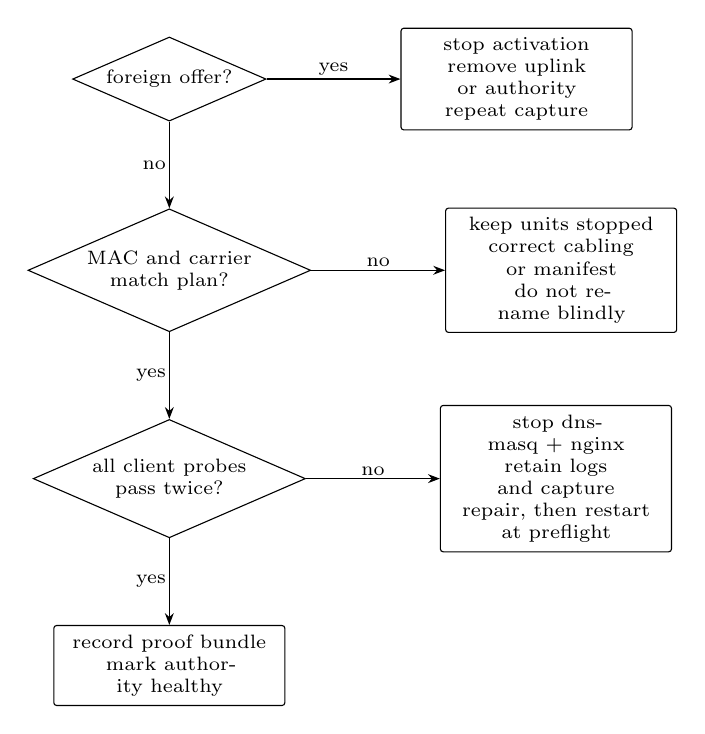
\begin{tikzpicture}[
  q/.style={draw,diamond,aspect=2.3,align=center,font=\scriptsize,
    inner sep=1.5pt},
  a/.style={draw,rounded corners=1pt,align=center,font=\scriptsize,
    text width=2.7cm,minimum height=.75cm},
  f/.style={-{Stealth[length=1.5mm]},line width=.55pt},
  lab/.style={font=\scriptsize,fill=white,inner sep=1pt}]
\node[q] (offer) {foreign offer?};
\node[a,right=17mm of offer] (isolate) {stop activation\\remove uplink or authority\\repeat capture};
\node[q,below=11mm of offer] (identity) {MAC and carrier\\match plan?};
\node[a,right=17mm of identity] (repair) {keep units stopped\\correct cabling or manifest\\do not rename blindly};
\node[q,below=11mm of identity] (probe) {all client probes\\pass twice?};
\node[a,right=17mm of probe] (bundle) {stop dnsmasq + nginx\\retain logs and capture\\repair, then restart at preflight};
\node[a,below=11mm of probe] (accept) {record proof bundle\\mark authority healthy};
\draw[f] (offer)--node[lab,above]{yes}(isolate);
\draw[f] (offer)--node[lab,left]{no}(identity);
\draw[f] (identity)--node[lab,above]{no}(repair);
\draw[f] (identity)--node[lab,left]{yes}(probe);
\draw[f] (probe)--node[lab,above]{no}(bundle);
\draw[f] (probe)--node[lab,left]{yes}(accept);
\end{tikzpicture}
\end{center}

Never ``test around'' a failed bundle member by leaving the other running. A
partial DHCP/DNS/PXE service is a failed Controller, and its evidence bundle
must retain the first failure rather than only the successful retry.

\section{Proof-bundle anatomy}
\begin{center}
\begin{tikzpicture}[
  node distance=5mm and 6mm,
  proof/.style={draw,rounded corners=1pt,text width=3.25cm,
    minimum height=.72cm,align=center,font=\scriptsize},
  link/.style={-{Stealth[length=1.5mm]},line width=.5pt}]
\node[proof] (inputs) {frozen inputs\\manifest · MAC · disk · subnet};
\node[proof,right=of inputs] (events) {ordered events\\boot · units · checkpoint · power};
\node[proof,right=of events] (observed) {external observations\\capture · lease · DNS · PXE};
\node[proof,below=of inputs] (state) {state identity\\UUIDs · subvolumes · artifact hashes};
\node[proof,right=of state] (failures) {first failures\\stderr · logs · rejected candidate};
\node[proof,right=of failures] (review) {review result\\explained diffs · operator sign-off};
\draw[link] (inputs)--(events);
\draw[link] (events)--(observed);
\draw[link] (state)--(failures);
\draw[link] (failures)--(review);
\draw[link] (inputs)--(state);
\draw[link] (observed)--(review);
\end{tikzpicture}
\end{center}
The bundle is complete only when it connects declared inputs to observations
made outside the Controller. Server logs corroborate client evidence; they do
not replace it. Secrets, passphrases and private key material never enter the
bundle.

\section{Optional roles}
\begin{telosfacts}[0.22]
\telosfact{Services}{Homebridge, openHAB and similar, as Podman quadlets with host networking --- required, because HomeKit and UPnP discovery depend on mDNS and do not survive bridged container networking. USB radios bound by stable \texttt{by-id} path. Application state on its own subvolume with its own backup, because its restore point is not the operating system's. Disabled by default. \governedby{ADR 0054}}
\telosfact{The trade-off}{Running Services on the Controller means a Controller maintenance window is also a home-automation outage. That is accepted and recorded, not hidden. When it stops being acceptable, the role moves to its own host and nothing else changes.}
\telosfact{Identity}{Samba AD DC in a VM --- a genuine separate trust boundary with its own restart and upgrade cadence, which is precisely when ADR 0014 permits a VM. Arch clients use SSSD's AD provider; Windows Pro clients domain-join; an AD-capable NAS can share the same identities. \governedby{ADR 0055}}
\telosfact{Break-glass}{Every managed machine keeps a separately named local administrator that is never a directory account. While the directory is down, only cached and break-glass logins work --- so this is mandatory, not a nicety.}
\end{telosfacts}

\section{Milestones}
\begin{telosfacts}[0.22]
\telosfact{A: functional proof}{Network boot, interactive authorization, install, isolated-network activation, DHCP and DNS validation, checkpoint and rollback, Workstation pivot. Encryption is real throughout. Secure Boot may be disabled under an explicit, recorded \texttt{development-proof} mode with manual LUKS2 unlock at every boot, no production data, and no custom signing material anywhere. \governedby{ADR 0043}}
\telosfact{B: hardening}{Revisit ADRs 0029--0042 as a group with operational experience, then enforce Secure Boot, implement signing and custody, enable TPM unlock only after its recovery path is tested, and prove an unattended cold restart restores service. Reprovision from the proven installer; the proof installation is disposable by construction. \governedby{ADR 0043}}
\telosfact{Known defects to fix in B}{The key separation in ADRs 0033--0035 is notional once ADR 0039 gives both media one passphrase; the backup's independence is defeated by sharing that passphrase; and ADR 0030's additive trust model may be infeasible on firmware that only permits \texttt{db} changes from Setup Mode. All three are recorded rather than rediscovered. \governedby{ADR 0057}}
\telosfact{No system passes}{Final acceptance until Milestone B is complete.}
\end{telosfacts}

\section{Measurable acceptance}
\begin{longtable}{@{}p{.22\linewidth}p{.31\linewidth}p{.41\linewidth}@{}}
\toprule
\textbf{Property} & \textbf{Threshold} & \textbf{Final proof}\\
\midrule
Bootstrap independence & Zero Controller-hosted prerequisites used during a bare-metal rebuild & Start with Controller powered off and storage unavailable; rebuild from offline instructions, installer and recorded inputs.\\
Network authority & Zero foreign offers; exactly one Controller offer per successful discovery & Timestamped capture spanning preflight and three client renewals, plus lease and DNS records.\\
Cold recovery & Three consecutive cold boots return DHCP, DNS and PXE without intervention after LUKS unlock in Milestone A & Power-event log and identical automated probe reports. Milestone B additionally requires the approved unattended unlock path.\\
Rollback & Failed system candidate reverted within 30 minutes; mutable service state neither rewound nor silently advanced by the rollback & Before/after checkpoint IDs, subvolume generations, probe report and application-state check.\\
Rebuild fidelity & Rebuilt manifest matches recorded role, disk, MAC and network inputs; every declared package/service difference is explained & Manifest diff, configuration diff, acceptance transcript and signed-off exceptions.\\
Safety boundary & No production data or production signing material on a \texttt{development-proof} system & Storage inventory and manifest-mode assertion included in the proof bundle.\\
\bottomrule
\end{longtable}

\begin{gate}{Final proof is a bundle, not a verdict}
Acceptance consists of the input manifest, cable/port record, preflight and
packet capture, checkpoint identifiers, cold-boot transcripts, client probe
results, recovery exercise and explained diffs. It passes only when a second
operator can trace every claimed boundary to an observation and reproduce the
probe without privileged knowledge.
\end{gate}

\begin{gate}{The bootstrap rule}
The Controller rebuild procedure must never require a functioning Controller to
obtain the instructions, DNS records, installer image, artifact manifest or
decryption material needed to rebuild it. Every recovery path in this design is
tested with the Controller assumed dead. That is the whole reason this document
is printable.
\end{gate}

\section{Final review worksheet}
\begin{tabularx}{\linewidth}{@{}p{.32\linewidth}L@{}}
\toprule
\textbf{Reviewer must answer} & \textbf{Evidence reference or disposition}\\
\midrule
Can the Controller be rebuilt while its disks, DNS and artifact service are unavailable? & Offline-media run ID, manifest digest and rebuild transcript:\\[3em]
Did any foreign DHCP authority answer during preflight or activation? & Capture file, interface and observation window:\\[3em]
Do client observations agree with server logs for lease, DNS and PXE? & Client probe report and correlated log interval:\\[3em]
Did three cold boots restore the same declared authority without configuration edits? & Power-event IDs and probe reports:\\[3em]
Did rollback preserve excluded mutable state and restore the named system checkpoint? & Before/after subvolume and checkpoint identities:\\[3em]
Are all differences, waivers and failed candidates retained rather than silently normalized? & Review record, owner and expiry:\\[3em]
\bottomrule
\end{tabularx}

\textbf{Disposition:}\quad
\fbox{\rule{0pt}{.8ex}\rule{.8ex}{0pt}} accept \qquad
\fbox{\rule{0pt}{.8ex}\rule{.8ex}{0pt}} reject \qquad
\fbox{\rule{0pt}{.8ex}\rule{.8ex}{0pt}} repeat named proof
\hfill Reviewer / date:\ \rule{3.1cm}{.4pt}
\end{document}

% leak test
